%%%%%%%%%%%%%%%%%%%%%%%%%%%%%%%%%%%%%%%%%%%%%%%%%%%%%%%%%%%
% Capitolo 5

\chapter{Modello dei dati di sistemi georeferenziali}
\label{modellodati}

Un \textit{modello dei dati} è un insieme di costrutti che descrivono e rappresentano particolari aspetti del mondo reale.
Esistono tre modelli dei dati che rappresentano diversi livelli di astrazione:
\begin{itemize}
\item \textbf{Modello concettuale}: descrive una selezione di oggetti e processi che caratterizzano un particolare problema.
\item \textbf{Modello logico}: descrive le entità e le relazioni definite nel modello concettuale, in modo orientato all'implementazione del sistema ed è espresso in forma di diagrammi e liste.
\item \textbf{Modello fisico}: descrive in dettaglio i file, gli archivi, le tabelle e definisce le relazioni tra queste ultime.
\end{itemize}

\begin{figure}
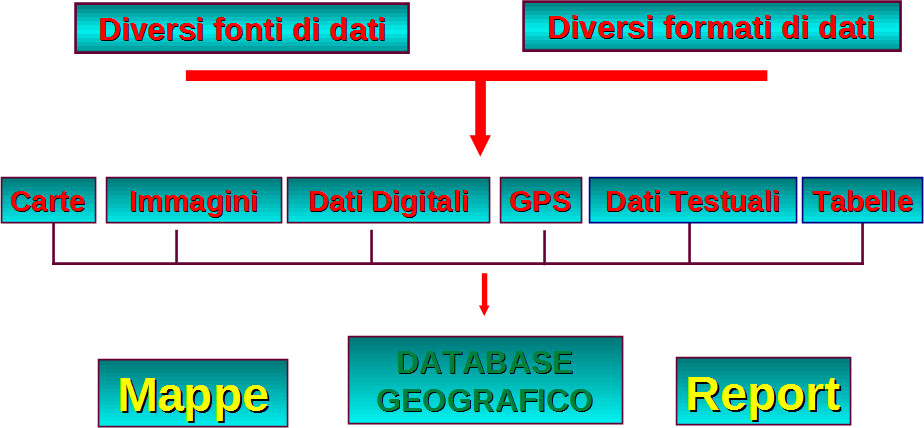
\includegraphics[scale=0.4]{./imgs/datigeograficiimage.jpg}
\caption{Utilizzo dati di un sistema georeferenziale\label{ref:datigeograficiimage}}

\end{figure}

%%%\section{Modello dati di un sistema georeferenziale}


Un sistema georeferenziale utilizza diverse fonti e diverse tipologie di dati, i quali possono essere carte, immagini, dati digitali, informazioni sul posizionamento, dati testuali, tabelle e che vanno a formare un \textbf{database geografico}, così come illustrato nella figura \ref{ref:datigeograficiimage}.

\section{I dati}
I dati geografici costruiscono il nostro modello di realtà. Essi si distinguono in:
\begin{itemize}
\item \textbf{Dati Spaziali} (Componente grafica)
\begin{itemize}
\item Raster
\item Vettoriali
\end{itemize}
\item \textbf{Dati attributo} (Componente tematica)
\begin{itemize}
\item Alfanumerici
\end{itemize}
\end{itemize}

\begin{figure}
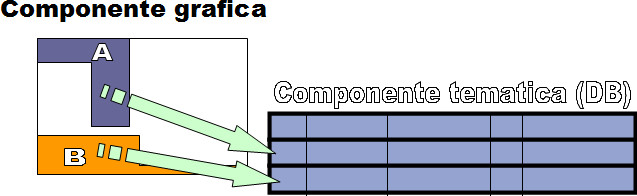
\includegraphics[scale=0.4]{./imgs/strutturedatigeograficiimage.jpg}
\caption{Struttura dei dati geografici\label{ref:strutturedatigeograficiimage}}
\end{figure}

Un sistema georeferenziale è in grado di gestire in modo integrato elementi grafici (dati spaziali) e tabelle dati (dati attributo).
Esso collega, infatti, dati spaziali (raster o vettoriali) a informazioni contenute in un database, che caratterizzano gli oggetti rappresentati (fig. \ref{ref:strutturedatigeograficiimage}).

\subsection{Dati vettoriali}
La struttura vettoriale individua elementi del territorio rappresentati fisicamente come:
\begin{itemize}
\item punti
\item linee
\item poligoni
\end{itemize}
Tali dati sino dati geometrici memorizzati attraverso le coordinate latitudine-longitudine dei punti e delle linee che li compongono.
La struttura vettoriale è indicata per descrivere elementi statici del territorio, con una propria dimensione e un proprio spazio geografico.

\subsection{Dati raster}
La struttura raster organizza i dati in una matrice di celle (quadrate, esagonali o triangolari), ognuna delle quali rappresentante uno specifico valore, che può essere di tipo grafico o descrittivo.
Tale struttura è utilizzata per rappresentare elementi continui.\\

I dati vettoriali e i dati raster, nel modello di un sistema georeferenziale, coesistono e si integrano a vicenda, ognuno con la propria utilità.


\section{Funzionalità}
Un sistema georeferenziale ha diverse funzionalità tutte connesse tra loro:
\begin{itemize}
\item \textbf{Acquisizione dati}
\item \textbf{Pre elaborazione}
\item \textbf{Gestione di banche dati}
\item \textbf{Analisi spaziale}
\item \textbf{Generazione di prodotti}
\end{itemize}

\subsubsection{Acquisizione dati}
Attività che prevede la raccolta, la predisposizione e l'acquisizione di informazioni geografiche.
Il dato può essere acquisito da banche dati già esistenti, da cartografie esistenti, da rilievi terrestri o aerei, da immagini satellitari.

\subsubsection{Pre-elaborazione}
Attività che prepara il sistema all'elaborazione vera e propria.
Consiste nella conversione dei formati, nella ricerca e correzione degli errori e nelle trasformazioni.

\subsubsection{Gestione di banche dati}
Attività che prevede il controllo di tutte le operazioni di accesso, inserimento, estrazione ed aggiornamento dei dati.
Solitamente per i sistemi georeferenziali è utilizzato un modello relazionale, in cui i dati sono concettualmente memorizzati come collezione di tabelle.
Alcuni campi comuni tra le tabelle sono utilizzati come \textit{chiave di relazione}.

\subsubsection{Analisi spaziale}
Funzionalità più importante e complessa di un sistema georeferenziale. Lo caratterizza in maniera univoca e lo differenzia da altri sistemi di informazione e trattamento dei dati.
Le principali funzioni sono:
\begin{itemize}
\item \textbf{query}: operazione di ricerca attraverso una grammatica predefinita per convenzioni e simboli.
\item \textbf{riclassificazione}: generazione nuovi attributi descrittivi partendo da uno o più attributi esistenti.
\item \textbf{aggregazione}: unione di più dati attributo e generazione di un nuovo attributo.
\item \textbf{sovrapposizione}: intersecazione di diversi strati informativi, tramite l'introduzione di punti, linee e poligoni su poligoni.
\item \textbf{analisi di rete}: funzioni che possono essere effettuate sulle reti, ovvero:
\begin{itemize}
\item ricerca del percorso minimo (o del minimo costo)
\item verifica della connettività tra due punti
\item allocazione di porzioni della rete
\end{itemize}
\end{itemize}

\subsubsection{Generazione di prodotti}
Attività di generazione dei prodotti finali, ovvero interfacce utente, report, carte e grafici, da restituire in formato cartaceo o digitale.

%%%%%%%%%%%%%%%%%%%%%%%%%%%%%%%%%%%%%%%%%%%%%%%%%%%%%%

\clearpage{\pagestyle{empty}\cleardoublepage}